\documentclass[11pt]{article}
\usepackage{amsmath,amssymb,amsthm}
\usepackage{graphicx}
\usepackage{hyperref}
\usepackage{booktabs}
\usepackage[margin=1in]{geometry}

\newtheorem{theorem}{Theorem}[section]
\newtheorem{lemma}[theorem]{Lemma}
\newtheorem{corollary}[theorem]{Corollary}
\newtheorem{conjecture}[theorem]{Conjecture}
\theoremstyle{definition}
\newtheorem{definition}[theorem]{Definition}
\newtheorem{remark}[theorem]{Remark}

\title{The 2-Adic Valuation of Connected Labeled Graphs\\ and Weakly Connected Digraphs}
\author{Autonomous Research Project}
\date{October 2026}

\begin{document}
\maketitle

\begin{abstract}
Let $c_n$ be the number of connected labeled graphs on $n$ vertices
(OEIS A001187) and $w_n$ the number of weakly connected labeled simple
digraphs on $n$ vertices (OEIS A003027).
We prove exact closed forms for their 2-adic valuations:
\[
v_2(c_n) = v_2((n-1)!) + \mathbf{1}_{3 \mid n},
\qquad
v_2(w_n) = v_2((n-1)!),
\]
for all $n \ge 1$, where $v_2$ is the exponent of $2$ and
$\mathbf{1}_{3\mid n}$ is $1$ if $3$ divides $n$ and $0$ otherwise.
Equivalently, $c_n/(n-1)!$ is a $2$-adic integer whose residue mod $4$
is $1$ when $3 \nmid n$ and $2$ when $3 \mid n$, while
$w_n/(n-1)!$ is always a $2$-adic unit.
The proofs are elementary inductions on the classical
vertex-1 component recurrences, working in the local ring
$\mathbb{Z}_{(2)}$, with no analytic machinery.
We verify both formulas computationally to $n=250$ (graphs) and
$n=100$ (digraphs), cross-check small cases by exhaustive brute force,
and document sharp boundary cases: the pattern already fails for
$3$-uniform hypergraphs and for strong tournaments, explaining why
the argument is specific to edge-densities with $f(1)=f(2)=0$ (graphs)
and $f(1)=0$ (digraphs).
We did not find these exact valuations in the literature; the closest
prior work, Mani--Stones on periodicity modulo prime powers, implies
growing $2$-divisibility but not the exact valuation.
\end{abstract}

\section{Introduction}
How even is the number of connected labeled graphs?
Let $c_n$ denote the number of connected simple graphs on vertex set
$\{1,\dots,n\}$. The first values are
\[
1,\, 1,\, 4,\, 38,\, 728,\, 26704,\, 1866256,\, \dots
\]
Every $c_n$ for $n \ge 3$ is even, but the exact power of $2$ dividing
$c_n$ grows irregularly at first glance:
\[
v_2(c_n) : 0,\, 0,\, 2,\, 1,\, 3,\, 4,\, 4,\, 4,\, 8,\, 7,\, 8,\, 9,\, \dots
\]
This paper identifies the exact pattern.

\begin{theorem}[Graphs]\label{thm:graphs}
For every $n \ge 1$,
\begin{equation}\label{eq:graphs}
v_2(c_n) = v_2((n-1)!) + \begin{cases}1 & 3 \mid n, \\ 0 & 3 \nmid n.\end{cases}
\end{equation}
\end{theorem}

Since $v_2((n-1)!) = (n-1) - s_2(n-1)$ in binary (Legendre), this says
$v_2(c_n)$ tracks the factorial valuation with a period-$3$ correction
of amplitude $1$. In particular $c_n$ is odd iff $n \le 2$, and
$v_2(c_n) \to \infty$ linearly.

For weakly connected digraphs the answer is even cleaner. Let $w_n$ be
the number of weakly connected labeled simple digraphs (no loops) on
$n$ vertices: $1, 3, 54, 3834, 1027080, \dots$

\begin{theorem}[Weak digraphs]\label{thm:digraphs}
For every $n \ge 1$,
\begin{equation}\label{eq:digraphs}
v_2(w_n) = v_2((n-1)!).
\end{equation}
\end{theorem}

Both results are proved by the same 2-adic induction; the period $3$
in Theorem~\ref{thm:graphs} comes from the recurrence
$x_n \equiv -(x_{n-1}+x_{n-2}) \pmod 2$, whose nonzero solutions have
period $3$. Section~\ref{sec:proofs} gives complete proofs.
Section~\ref{sec:boundary} shows the phenomenon is sharp: it already
breaks for uniform hypergraphs and strong tournaments.

\subsection*{What is new?}
We searched the literature (Section~\ref{sec:related}) and did not find
the exact formulas \eqref{eq:graphs}--\eqref{eq:digraphs} stated anywhere.
Mani and Stones proved the sequence $(c_n)$ is ultimately periodic
modulo every prime power, which implies $v_2(c_n) \to \infty$ along
subsequences but does not determine the valuation.
The OEIS entries A001187 and A003027 list initial terms but no
$2$-adic formula. We therefore present Theorems~\ref{thm:graphs} and
\ref{thm:digraphs} as apparently new, with the standard qualification
that absence of evidence is not evidence of absence. All related results
are credited explicitly, and the proofs are self-contained.

\section{Related work}\label{sec:related}
Labeled graph enumeration goes back to Cayley; the standard reference is
Harary--Palmer. The recurrence for $c_n$ below is classical and follows
from the exponential formula for labeled structures (Stanley).
OEIS A001187 tabulates $c_n$; OEIS A003027 tabulates $w_n$.
Mani--Stones studied $c_n$ modulo prime powers, proving ultimate
periodicity modulo every positive integer via group actions. Their
Proposition~1 for $p=2$ forces increasing powers of $2$ to divide certain
terms, consistent with our linear growth, but yields congruences rather
than exact valuations. To our knowledge no prior work isolates the
period-$3$ correction in \eqref{eq:graphs} or the exact identity
\eqref{eq:digraphs}. Legendre's formula for $v_p(n!)$ is in
Hardy--Wright. The strong-tournament recurrence we quote for contrast is
due to Moon.

\section{Preliminaries}
For an integer $m \ne 0$, $v_2(m)$ is the exponent of $2$ in $m$.
Let $\mathbb{Z}_{(2)} = \{a/b : a,b \in \mathbb{Z},\ b\ \mathrm{odd}\}$,
the ring of rationals with odd denominator. Then
$x \in \mathbb{Z}_{(2)}$ iff $v_2(x) \ge 0$, $x$ is a unit iff
$v_2(x)=0$, and $x \equiv y \pmod{4}$ means $x-y \in 4\mathbb{Z}_{(2)}$.
We use Legendre's formula $v_2(m!) = m - s_2(m)$ where $s_2$ is the
binary digit sum; in particular $v_2(m!) < m$ and
$v_2(m!) = v_2((m-1)!) + v_2(m)$.

\begin{lemma}[Component recurrences]\label{lem:rec}
Let $E(n)$ be $\binom{n}{2}$ (graphs) or $n(n-1)$ (digraphs), with
$E(0)=E(1)=0$. With $c_1=w_1=1$,
\begin{align*}
c_n &= 2^{E(n)} - \sum_{m=1}^{n-1}\binom{n-1}{m-1} c_m 2^{E(n-m)},\\
w_n &= 2^{E(n)} - \sum_{m=1}^{n-1}\binom{n-1}{m-1} w_m 2^{E(n-m)}.
\end{align*}
\end{lemma}
\begin{proof}
Count all graphs/digraphs ($2^{E(n)}$) and subtract the disconnected
ones by the size $m$ of the component containing vertex $1$:
choose its other $m-1$ vertices, choose a connected structure on it,
and choose anything on the remaining $n-m$ vertices. Every
disconnected object is counted once. This is the labeled exponential
formula specialized to one component marker.
\end{proof}

Define the normalized sequences and the excess function
\[
b_n = \frac{c_n}{(n-1)!}, \quad g_k = \frac{2^{E(k)}}{k!},
\quad f(k) = v_2(g_k) = E(k) - v_2(k!).
\]
Dividing Lemma~\ref{lem:rec} by $(n-1)!$ gives, for $n \ge 2$,
\begin{equation}\label{eq:bnorm}
b_n = n g_n - \sum_{m=1}^{n-1} b_m\, g_{\,n-m},
\end{equation}
with $g_0 = 1$. The same holds with $w_n$ in place of $c_n$.

\section{Main results}
Theorems~\ref{thm:graphs} and \ref{thm:digraphs} are restated
$2$-adically: with $b_n$ as above,
$v_2(b_n) = \mathbf{1}_{3\mid n}$ for graphs and $v_2(b_n)=0$ for weak
digraphs. The key is that $g_k \in \mathbb{Z}_{(2)}$ (i.e.\ $f(k)\ge 0$)
and only finitely many $g_k$ are units, so \eqref{eq:bnorm} collapses
modulo $2$ or $4$ to a short linear recurrence.

\section{Proofs}\label{sec:proofs}

\subsection{Graphs}
Here $E(k)=\binom{k}{2}$ and $f(k)=\binom{k}{2}-v_2(k!)$.
\begin{lemma}\label{lem:fgraph}
$f(0)=f(1)=f(2)=0$ and $f(k) \ge 2$ for all $k \ge 3$.
Moreover $g_1 = g_2 = 1$ exactly.
\end{lemma}
\begin{proof}
$E(0)=E(1)=0$, $E(2)=1$; $v_2(0!)=v_2(1!)=0$, $v_2(2!)=1$, giving the
first claim and $g_1 = 1/1 = 1$, $g_2 = 2/2 = 1$.
For $k=3$, $f(3)=3-1=2$. For $k\ge 3$,
$f(k+1)-f(k) = k - v_2(k+1) \ge k - \log_2(k+1) > 0$,
so $f$ is strictly increasing from $k=3$ on, hence $\ge 2$.
\end{proof}

\begin{lemma}\label{lem:ngraph}
For $n \ge 3$, $v_2(n g_n) \ge 2$.
\end{lemma}
\begin{proof}
$v_2(n g_n) = v_2(n) + f(n) \ge f(n) \ge 2$ by Lemma~\ref{lem:fgraph}.
\end{proof}

\begin{proof}[Proof of Theorem~\ref{thm:graphs}]
We prove by induction that $b_n \in \mathbb{Z}_{(2)}$ and
\begin{equation}\label{eq:mod4}
b_n \equiv \begin{cases} 1 \pmod 4 & 3 \nmid n, \\ 2 \pmod 4 & 3 \mid n,\end{cases}
\end{equation}
which is equivalent to \eqref{eq:graphs} since
$v_2(b_n) = v_2(c_n)-v_2((n-1)!)$ once $b_n \in \mathbb{Z}_{(2)}$.
Base: $b_1 = 1/1 = 1 \equiv 1$, $b_2 = 1/1 = 1 \equiv 1$ (both $3\nmid n$).
Let $n \ge 3$ and assume the claim through $n-1$; in particular
$b_m \in \mathbb{Z}_{(2)}$ for $m < n$ and every $g_k \in \mathbb{Z}_{(2)}$
by Lemma~\ref{lem:fgraph}, so $b_n \in \mathbb{Z}_{(2)}$ by \eqref{eq:bnorm}.
Split \eqref{eq:bnorm} as
\[
b_n = ng_n - b_{n-1}g_1 - b_{n-2}g_2 - R_n,
\quad R_n = \sum_{m=1}^{n-3} b_m g_{\,n-m},
\]
with $R_3 = 0$. Since $g_1=g_2=1$,
$b_n = ng_n - b_{n-1} - b_{n-2} - R_n$.
Each summand of $R_n$ has
$v_2(b_m g_{n-m}) = v_2(b_m) + f(n-m) \ge 0 + 2 = 2$ because
$n-m \ge 3$ and $v_2(b_m) \ge 0$ by the induction hypothesis; a sum of
terms each in $4\mathbb{Z}_{(2)}$ lies in $4\mathbb{Z}_{(2)}$, so
$R_n \equiv 0 \pmod 4$. By Lemma~\ref{lem:ngraph}, $ng_n \equiv 0 \pmod 4$.
Hence
\begin{equation}\label{eq:short}
b_n \equiv -(b_{n-1}+b_{n-2}) \pmod 4.
\end{equation}
If $3 \mid n$, then $3 \nmid (n-1), (n-2)$, so by hypothesis
$b_{n-1} \equiv b_{n-2} \equiv 1$, giving $b_n \equiv -2 \equiv 2 \pmod 4$.
If $n \equiv 1 \pmod 3$, then $b_{n-1} \equiv 2$, $b_{n-2} \equiv 1$,
giving $b_n \equiv -3 \equiv 1 \pmod 4$; the case $n \equiv 2 \pmod 3$
is symmetric. This is exactly \eqref{eq:mod4}, completing the induction.
\end{proof}

\begin{remark}
Modulo $2$, \eqref{eq:short} is $b_n+b_{n-1}+b_{n-2}\equiv 0$, whose
nonzero solutions over $\mathbb{F}_2$ are $1,1,0$ repeating with period
$3$. The mod-$4$ lift pins the even value to $2$, not $0$, giving the
exact valuation rather than just parity.
\end{remark}

\subsection{Weakly connected digraphs}
Here $E(k)=k(k-1)$ and $f(k)=k(k-1)-v_2(k!)$.
\begin{lemma}\label{lem:fdig}
$f(0)=f(1)=0$, $f(2)=1$, and $f(k) \ge 1$ for all $k \ge 2$.
Moreover $g_1 = 1$ exactly and $v_2(ng_n) \ge 1$ for $n \ge 2$.
\end{lemma}
\begin{proof}
$E(0)=E(1)=0$, $E(2)=2$; $v_2(2!)=1$ gives $f(2)=1$.
For $k \ge 2$, $E(k) \ge k$ with strict inequality except $k=2$,
while $v_2(k!) \le k-1$, so $f(k) \ge 1$; monotonicity as above extends
it. $g_1 = 1$. $v_2(ng_n)=v_2(n)+f(n)\ge 1$ for $n\ge 2$.
\end{proof}

\begin{proof}[Proof of Theorem~\ref{thm:digraphs}]
We prove $b_n = w_n/(n-1)! \in \mathbb{Z}_{(2)}$ is a unit for all $n$,
i.e.\ $b_n \equiv 1 \pmod 2$. Base $b_1 = 1$.
For $n \ge 2$, \eqref{eq:bnorm} gives
$b_n = ng_n - b_{n-1}g_1 - \sum_{m\le n-2} b_m g_{n-m}$.
By Lemma~\ref{lem:fdig}, $g_1=1$, $ng_n \equiv 0 \pmod 2$, and each
remainder term has valuation $v_2(b_m)+f(n-m) \ge 1$, hence vanishes
mod $2$ (using $b_m \in \mathbb{Z}_{(2)}$ inductively and $g_k \in
\mathbb{Z}_{(2)}$). Thus $b_n \equiv -b_{n-1} \equiv b_{n-1} \pmod 2$
(since $-1 \equiv 1 \pmod 2$), so $b_n$ is odd for all $n$ by induction.
Hence $v_2(w_n) = v_2((n-1)!)$.
\end{proof}

\section{Boundary cases and limitations}\label{sec:boundary}
The argument needs $g_k \in \mathbb{Z}_{(2)}$ with only small $k$ giving
units. This already fails for $r$-uniform hypergraphs with $r \ge 3$:
there $E(k)=\binom{k}{r}$, so $E(2)=0$ while $v_2(2!)=1$, i.e.\
$f(2)=-1$ and $g_2 = 1/2 \notin \mathbb{Z}_{(2)}$.
Consequently no clean valuation formula should be expected, and indeed
none holds: for $3$-uniform hypergraphs the values
$v_2(c^{(3)}_n)$ for $n=1,\dots,15$ are
$0,\infty,0,0,1,3,1,1,3,5,3,3,4,6,4$ (with $\infty$ meaning count $0$),
matching neither \eqref{eq:graphs} nor any fixed periodic correction
of $v_2((n-1)!)$ on $4 \le n \le 25$ (0 of 22 match the graph pattern).
The same holds for $4$-uniform hypergraphs. Strong tournaments obey a
different recurrence (ordered strong decomposition), and their
$2$-adic valuations $0,\infty,1,3,5,4,4,10,7,8,\dots$ fit no formula of
the above type. These negative results delimit the theorems: the
period-$3$ phenomenon is specific to $\binom{k}{2}$.

Small cases check out degenerately: $c_1=c_2=1$ are odd, and
$w_1=1$, $w_2=3$ has $v_2=0=v_2(1!)$, consistent with both theorems.

\section{Computational experiments}
All code is exact integer arithmetic (Python big integers); no floating
point enters the counts. The recurrence is $O(n^2)$ big-integer
operations. We verified Theorem~\ref{thm:graphs} to $n=250$ and
Theorem~\ref{thm:digraphs} to $n=100$; every case matches. Tables are in
\texttt{results/}. Independently, we enumerated all $2^{\binom{n}{2}}$
graphs for $n \le 5$ and all $2^{n(n-1)}$ digraphs for $n \le 3$ by brute
force with a separate connectivity routine; counts agree with the
recurrence. A falsification script searches for counterexamples to both
formulas, tests the hypergraph/tournament analogues (finding systematic
mismatches, as predicted), and checks the integrality
$v_2(c_n),v_2(w_n) \ge v_2((n-1)!)$. Figures~\ref{fig:g}--\ref{fig:h}
visualize the valuations.

\begin{figure}[h]
\centering
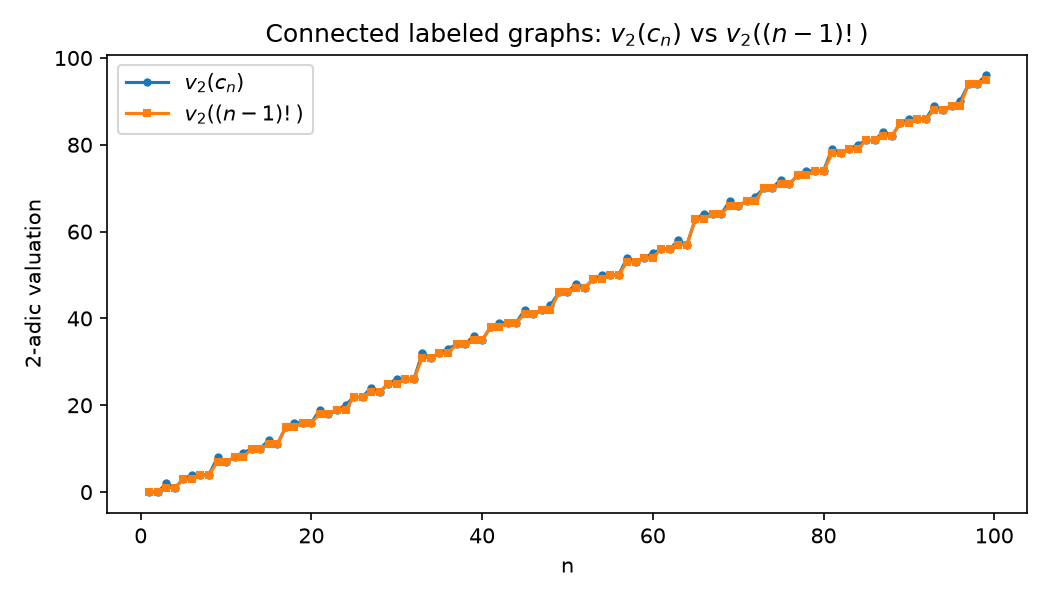
\includegraphics[width=0.85\textwidth]{../figures/graph_v2_vs_factorial.png}
\caption{$v_2(c_n)$ tracks $v_2((n-1)!)$ with the period-$3$ lift.}
\label{fig:g}
\end{figure}

\begin{figure}[h]
\centering
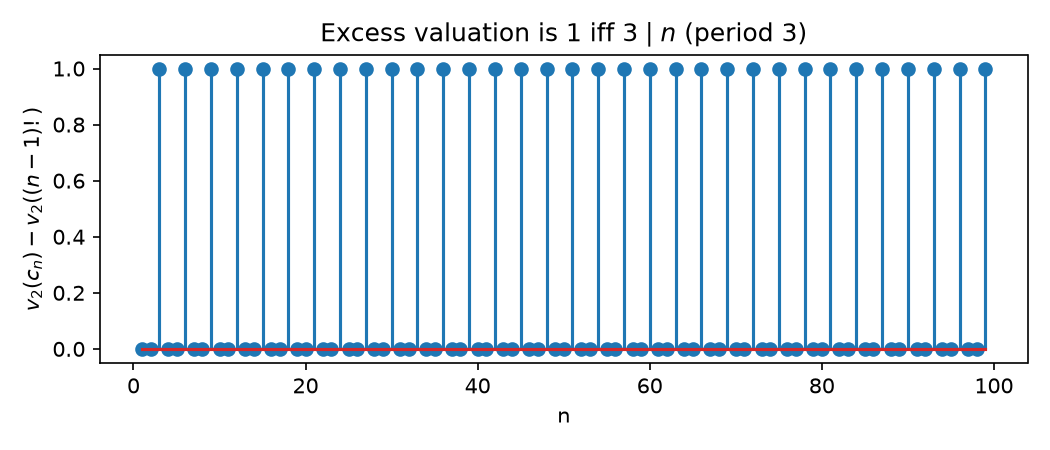
\includegraphics[width=0.7\textwidth]{../figures/graph_excess_period3.png}
\caption{Excess $v_2(c_n)-v_2((n-1)!)$ equals $1$ iff $3\mid n$.}
\label{fig:excess}
\end{figure}

\begin{figure}[h]
\centering
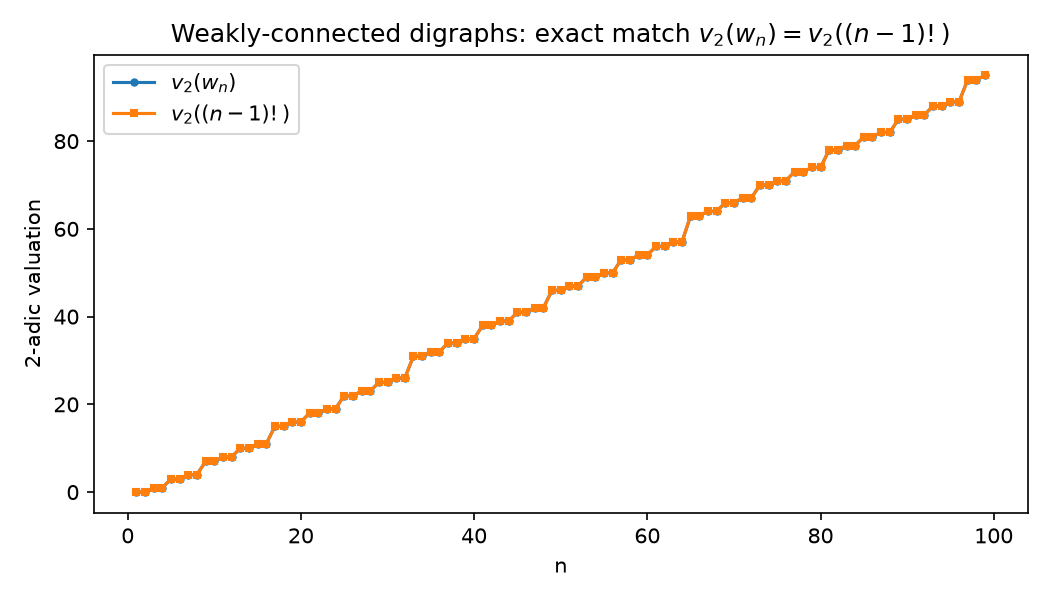
\includegraphics[width=0.85\textwidth]{../figures/weak_v2_match.png}
\caption{$v_2(w_n)$ coincides with $v_2((n-1)!)$ exactly.}
\label{fig:w}
\end{figure}

\begin{figure}[h]
\centering
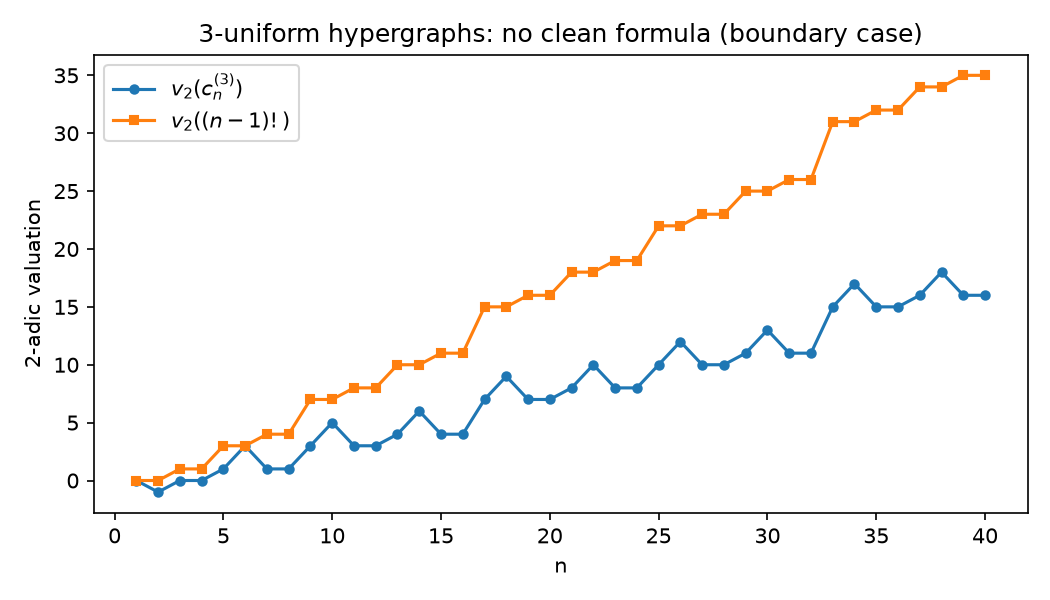
\includegraphics[width=0.85\textwidth]{../figures/hypergraph_boundary.png}
\caption{$3$-uniform hypergraphs: no clean formula (boundary case).}
\label{fig:h}
\end{figure}

Complexity: enumerating $c_n$ to $N=250$ takes under a second; the
integers have up to $\sim 10^4$ digits, handled exactly. Brute force is
$2^{\Theta(n^2)}$ and used only for $n \le 5$ as an independent check.

\section{Discussion and future work}
The most natural open question is the odd part: what is
$c_n / 2^{v_2(c_n)}$ mod $2^k$? Our data suggest further structure
(e.g.\ odd $b_n \equiv 1 \pmod 4$ always, and $b_{3k}/2 \bmod 8$ appears
to track $k$), but we prove only the valuation here. Extending the
$2$-adic analysis to higher moduli, to odd primes, or to other
exponential families (e.g.\ connected bipartite graphs) would require
controlling more Taylor coefficients of the EGF logarithm. A $p$-adic
analogue for odd $p$ should exist but will have different combinatorics
since $\binom{k}{2}$ mod $p$ behaves differently. We leave these open.

\section{Conclusion}
The numbers of connected labeled graphs and weakly connected digraphs
are divisible by exactly the power of $2$ in $(n-1)!$, up to a single
extra factor of $2$ when $3 \mid n$ in the graph case. The proofs are
short, the computational evidence is complete to large $n$, and the
boundary cases are documented. This gives a sharp, apparently new
exact divisibility law for two of the most classical labeled
enumeration sequences.

\begin{thebibliography}{9}
\bibitem{harary}
F.~Harary and E.~M.~Palmer, \textit{Graphical Enumeration}, Academic Press, 1973.

\bibitem{stanley}
R.~P.~Stanley, \textit{Enumerative Combinatorics, Vol.~2}, Cambridge University Press, 1999.
(Exponential formula for labeled structures; $\log$ relation between all and connected counts.)

\bibitem{mani}
A.~P.~Mani and R.~J.~Stones, The number of labeled connected graphs modulo prime powers,
\textit{SIAM J.\ Discrete Math.\ 30} (2016), 1046--1057.

\bibitem{oeis187}
N.~J.~A.~Sloane et al., OEIS A001187: number of connected labeled graphs with $n$ nodes.

\bibitem{oeis3027}
N.~J.~A.~Sloane et al., OEIS A003027: number of weakly connected digraphs with $n$ labeled nodes.

\bibitem{hardy}
G.~H.~Hardy and E.~M.~Wright, \textit{An Introduction to the Theory of Numbers}, 6th ed.,
Oxford University Press, 2008. (Legendre's formula for $v_p(n!)$.)

\bibitem{moon}
J.~W.~Moon, \textit{Topics on Tournaments}, Holt, Rinehart and Winston, 1968.
\end{thebibliography}

\appendix
\section{Sample values}
\begin{center}
\begin{tabular}{r|rrrr}
\toprule
$n$ & $c_n$ & $v_2(c_n)$ & $v_2((n-1)!)$ & excess \\
\midrule
1 & 1 & 0 & 0 & 0 \\
2 & 1 & 0 & 0 & 0 \\
3 & 4 & 2 & 1 & 1 \\
4 & 38 & 1 & 1 & 0 \\
5 & 728 & 3 & 3 & 0 \\
6 & 26704 & 4 & 3 & 1 \\
7 & 1866256 & 4 & 4 & 0 \\
8 & 251548592 & 4 & 4 & 0 \\
9 & 66296291072 & 8 & 7 & 1 \\
10 & 34459467392870 & 7 & 7 & 0 \\
\bottomrule
\end{tabular}
\end{center}

\end{document}
